\documentclass{beamer}
\usetheme{Boadilla}

\usepackage{amsmath}
\usepackage{amsfonts}
\usepackage{hyperref}

\usepackage{amsmath}
\DeclareMathOperator*{\argmax}{arg\,max}
\DeclareMathOperator*{\argmin}{arg\,min}

\title{Learning Approximately Objective Priors}
\author{Galina Boeva}
\institute{MIPT, 2023}


\begin{document}

\begin{frame}
    \titlepage
\end{frame}


\begin{frame}
    \tableofcontents
\end{frame}


\section{Motivation}
\begin{frame}{Motivation}
    \begin{block}{Main idea}
    It's difficult to have informative priors, so they turn to uninformative priors, but for many models it's impossible to deduce them. Therefore, the authors propose to approximate these prior.
    \end{block} 
\end{frame}

\section{Definition}
\begin{frame}{Definition}
    \begin{block}{Likelihood}
    \begin{equation}
        p(\mathcal{D}|\theta) = \displaystyle\prod_{i=1}^N p(x_i|\theta),
    \end{equation} 
        where $\theta$ are the model parameters and $\mathcal{D}$ is the dataset, which is comporised of N i.i.d. observations $x_i \in \mathcal{X}$. $p(\theta)$ denotes the prior, $p(\theta|\mathcal{D})$ the posterior, and $p(\mathcal{D}) =\int\limits_{\theta} p(\mathcal{D}|\theta)p(\theta)d\theta$ the marginal likelihood.
    \end{block}
    \begin{block}{Reference prior}
    Reference prior is the distribution that maximizes the mutual information between the parameters $\theta$ and the data $\mathcal{D}$:
    \begin{equation}
        p^{*}(\theta) = \displaystyle \argmax_{p(\theta)} \mathbb{I}(\theta, \mathcal{D}) = \displaystyle\argmax_{p(\theta)} \mathbb{H}[\theta]  - \mathbb{H}[\theta | \mathcal{D}]
    \end{equation}
    \end{block}
\end{frame}

\begin{frame}{Definition}
    \begin{block}{Mutual information}
    Mutual information in terms of a Kullback-Leibler divergence:
    \begin{equation}
        I(\theta, \mathcal{D}) = \int\limits_{\mathcal{D}} p(\mathcal{D}) KLD[p(\theta|\mathcal{D}) || p(\theta)] d\mathcal{D}.
    \end{equation} 
    \begin{equation}
        I(\theta, \mathcal{D}) = - \int\limits_{\theta} p(\theta) \log \frac{p(\theta)}{f(\theta)} d\theta,  
        f(\theta) = \exp\Big\{\int\limits_{\mathcal{D}} p(\mathcal{D}|\theta) \log p(\theta|\mathcal{D}) d\mathcal{D}\Big\}.
    \end{equation} 
    \end{block}
    \begin{block}{Jeffreys Prior}
    \begin{equation}
        \pi(\theta) \propto \sqrt{det \mathcal{F}[\theta]}.
    \end{equation} 
    \end{block}
    \begin{block}{Bernstein Von Mises theorem}
    \begin{equation}
    p(\theta|\mathcal{D}) \approx N(\theta_{MLE}, \mathcal{F}^{-1}(\theta))
    \end{equation} 
    \end{block}
    
\end{frame}


\section{Methods}
\begin{frame}{Information lower bound}
\centering
\begin{block}{Argmax $\lambda$}
    \[
    \boldsymbol{\lambda}_{*} = \displaystyle \argmax_{\boldsymbol{\lambda}} \mathbb{I} (\boldsymbol{\theta}, \mathcal{D})
    = \displaystyle\argmax_{\boldsymbol{\lambda}}  \int\limits_{\boldsymbol{\theta}} p_{\boldsymbol{\lambda}}(\boldsymbol{\theta}) \int\limits_{\mathcal{D}} p(\mathcal{D}|\boldsymbol{\theta}) \log \frac{p(\mathcal{D}, \boldsymbol{\theta})}{p_{\boldsymbol{\lambda}}(\boldsymbol{\theta})p(\mathcal{D})} d\mathcal{D}d\boldsymbol{\theta} \]
    \[
    = \displaystyle\argmax_{\boldsymbol{\lambda}}  \int\limits_{\boldsymbol{\theta}} p_{\boldsymbol{\lambda}}(\boldsymbol{\theta}) \int\limits_{\mathcal{D}} p(\mathcal{D}|\boldsymbol{\theta}) \log \frac{p(\mathcal{D}, \boldsymbol{\theta})}{p(\mathcal{D})} d\mathcal{D} d\boldsymbol{\theta} =\] 
    \begin{equation}
    = \displaystyle\argmax_{\boldsymbol{\lambda}} \mathbb{E}_{\boldsymbol{\theta}_{\boldsymbol{\lambda}}} [-\mathbb{H}_{\mathcal{D}|\boldsymbol{\theta}}[\mathcal{D}] - \mathbb{E}_{\mathcal{D}|\boldsymbol{\theta}}[\log p(\mathcal{D})]]
    \end{equation}
    \end{block}
    
    \begin{block}{Bounding $\log p(\mathcal{D})$}
    Using variational Renyi bound:
    \begin{equation}
        \log p(\mathcal{D}) \leq \frac{1}{1 - \alpha} \log \mathbb{E}_{\boldsymbol{\theta}}(p(\mathcal{D}|\boldsymbol{\theta})^{(1 - \alpha)}), \alpha \leq 0. 
    \end{equation}
        
    \end{block}
 
\end{frame}

\begin{frame}{Information lower bound}
\centering
%\begin{block}{Lower bound for mutual information}
\begin{block}{Lower bound for $\lambda$} 
    \begin{equation}
        \mathbb{I}(\theta, \mathcal{D}) \geq \mathbb{E}_{\boldsymbol{\theta}_{\boldsymbol{\lambda}}}\Big[ -\mathbb{H}_{\mathcal{D}|\theta}[\mathcal{D}] - \frac{1}{1 - \alpha} \log \mathbb{E}_{\boldsymbol{\theta}}[p(\mathcal{D}|\theta)^{1 - \alpha}]\Big].
    \end{equation}

    \begin{equation}
    \mathbb{I}(\theta, \mathcal{D}) \geq \mathbb{J}_{\mathcal{RP}}(\boldsymbol{\lambda}) = \mathbb{E}_{\boldsymbol{\theta}_{\boldsymbol{\lambda}}}\Big[-\mathbb{H}_{\mathcal{D}|\theta}[\mathcal{D}] - \mathbb{E}_{\mathcal{D}|\theta}[\displaystyle \max_s \log p(\mathcal{D}|\boldsymbol{\hat{\theta}}_{s})]\Big].
    \end{equation}
    \begin{equation}
    \mathbb{J}_{\mathcal{RP}}(\boldsymbol{\lambda}) = \mathbb{E}_{\boldsymbol{\theta}_{\boldsymbol{\lambda}}} \mathbb{E}_{\mathcal{D}|\boldsymbol{\theta}} \Big[\log p(\mathcal{D}|\boldsymbol{\theta}) - \displaystyle \max_s \log p(\mathcal{D}|\boldsymbol{\hat{\theta}}_{s})\Big].
    \end{equation}
    
    \[\mathbb{\hat{J}}_{\mathcal{RP}}(\boldsymbol{\lambda})= \frac{1}{S}\sum^{S}_{s=1} \mathbb{H}[p(\mathcal{D}|\boldsymbol{\hat{\theta}}_{s})||p(\mathcal{D}|\boldsymbol{\hat{\theta}}_{s})] - \mathbb{H}_{\mathcal{D}|\boldsymbol{\hat{\theta}}_{s}}[\mathcal{D}] = \]
    \begin{equation}
     = \frac{1}{S} \sum^{S}_{s=1} KLD[p(\mathcal{D}|\boldsymbol{\hat{\theta}}_{s})||p(\mathcal{D}|\boldsymbol{\hat{\theta}}_{s})]
    \end{equation}
    \end{block} 
  
\end{frame}

\begin{frame}{Particle descent}
\begin{block}{Stein Variational Gradient Descent}
\[\bar{\theta}^{t+1}_j = \bar{\theta}^t_j + \eta \phi[\theta]\]
\[\phi[\theta] = \frac{1}{K} \sum^K_{k=1} \kappa(\bar{\theta}^t_k, \bar{\theta}^t_j)\nabla_{\bar{\theta}_k} \log p(\bar{\theta}^t_k) + \nabla_{\bar{\theta}_k} \kappa(\bar{\theta}^t_k, \bar{\theta}^t_j).\]
 
\end{block}
\begin{block}{A-SVGD for RP Approximations}
\[\nabla \bar{\theta} \log f(\bar{\theta}) = \nabla_{\bar{\theta}} \int\limits_{\mathcal{D}} p(\mathcal{D}|\bar{\theta}) \log p(\bar{\theta}|\mathcal{D}) d\mathcal{D} = \]
\[= \int\limits_{\mathcal{D}} p(\mathcal{D}|\bar{\theta}) \log \frac{p(\mathcal{D}|\bar{\theta}) \mathds{1}_{\Theta}}{p(\mathcal{D})} d\mathcal{D} = -\nabla_{\bar{\theta}} \mathbb{H}_{\mathcal{D}|\bar{\theta}}[\mathcal{D}] - \nabla_{\bar{\theta}} \mathbb{E}_{\mathcal{D}|\bar{\theta}}[\log p(\mathcal{D})]\]
\[= \nabla_{\bar{\theta}} \frac{1}{S} \displaystyle \sum_s KLD[p(\mathcal{D}|\bar{\theta}) || p(\mathcal{D}|\hat{\theta}_s)].\]
\end{block}
     
\end{frame}



\section{Empirical results}
\begin{frame}{Empirical results: Approximation}
    \begin{figure}
        \centering
        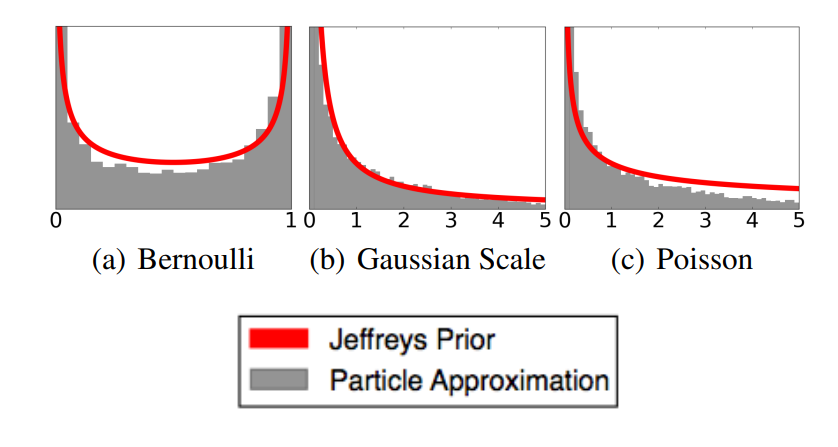
\includegraphics[scale=0.5]{images/bmm_preza.png}
        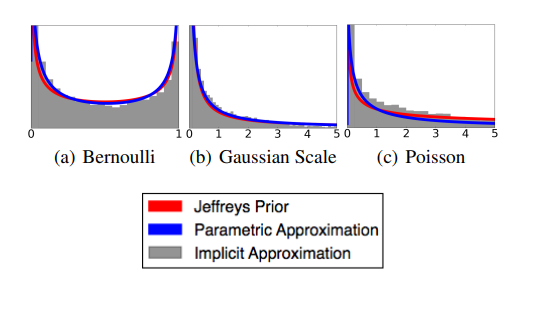
\includegraphics[scale=0.78]{images/bmm_3.png}
        \caption{Approximation via Particle Descent.}
        \label{fig:enter-label}
    \end{figure}
\end{frame}
\begin{frame}{Empirical results: Approximation Quality}
    \begin{figure}
        \centering
        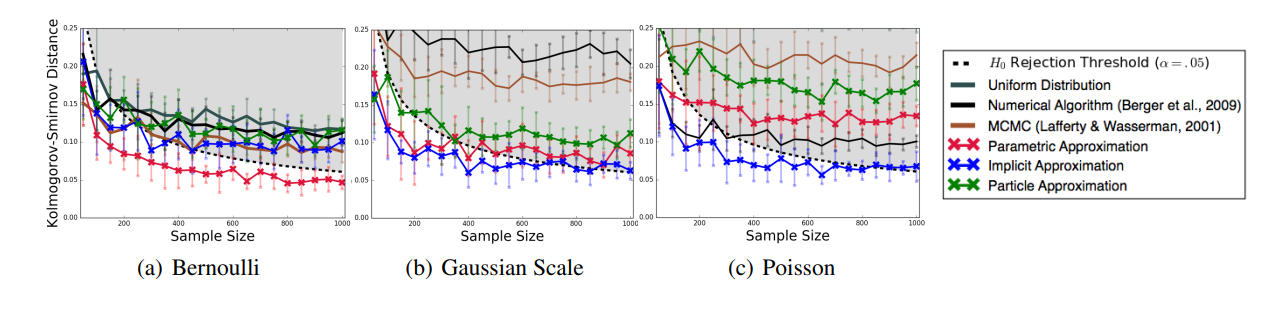
\includegraphics[scale=0.56]{images/bmm_preza_1.png}
        \caption{Quantifying the Approximation Quality.}
        \label{fig:enter-label}
    \end{figure}
\end{frame}

\begin{frame}{Empirical results: VAE}
    \begin{figure}
        \centering
        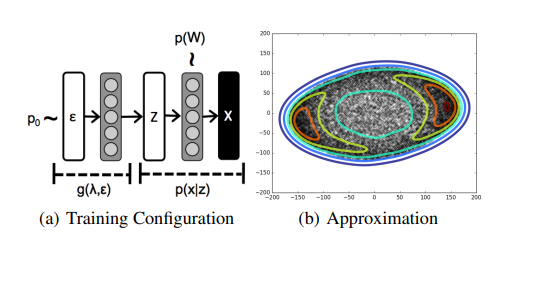
\includegraphics[scale=0.56]{images/bmm_preza_2.png}
        \caption{Learning the Variational Autoencoder’s Reference Prior. (a) computational pipeline from the implicit prior through the VAE decoder; (b) RP approximation (contours are generated via kernel density estimation on 10, 000 samples).}
        \label{fig:enter-label}
    \end{figure}
\end{frame}


\begin{frame}{Literature}
    \begin{enumerate}
        \item \textbf{Main article} \href{https://arxiv.org/pdf/1704.01168.pdf}
        {Learning Approximately Objective Priors}.
    \end{enumerate}
\end{frame}



\end{document}